% TAAI 2026 國內論文（英文版）——依中文修訂稿翻譯，版面依 TAAI 2026 國內論文組官方英文 Word 範本
% 投稿以同目錄 taai2026-domestic-full-paper-en.docx 為準：該檔直接以官方範本
%   https://taai2026.github.io/assets/downloads/template/taai2026-domestic-full-paper-template-en.docx
% 的樣式與分節建立，Word 排版為 6 頁。本檔與 .docx 文字相同，版面參數比照範本（A4、上 35 mm、下 30 mm、
% 左 19 mm、右 22.9 mm、雙欄間距 8 mm、內文 10 pt Times New Roman、題目 14 pt 粗體全大寫、第一層標題全大寫置中、
% 圖說「Fig. 1.」在圖下、表說「Table 1.」在表上、無頁碼），以 XeLaTeX 編譯；斷行與分頁未必與 Word 相同。
% 數字、引用與參考文獻與中文版逐段相同；翻譯與排版說明見同目錄〈論文修訂說明.md〉；圖檔在 Image/論文修訂說明/。
% 各小節的數據來源註解沿用中文版（taai2026-domestic-full-paper.tex）。
\documentclass[10pt,twocolumn,a4paper]{article}
\usepackage{fontspec}
\IfFontExistsTF{Times New Roman}{\setmainfont{Times New Roman}}{\setmainfont{TeX Gyre Termes}}
\usepackage[a4paper,top=35mm,bottom=30mm,left=19mm,right=22.9mm,columnsep=8mm]{geometry}
\usepackage{graphicx}
\graphicspath{{Image/論文修訂說明/}}
\usepackage{booktabs}
\usepackage{cite}
\usepackage{caption}
\usepackage{titlesec}
\usepackage{flushend}
\usepackage[hidelinks]{hyperref}

\pagestyle{empty}
\setlength{\parindent}{0.25in}
\setlength{\parskip}{0pt}

% 第一層標題：全大寫、粗體、置中，前後各空一行；第二層：粗體、靠左，形如「2.1.」
\titleformat{\section}{\normalfont\normalsize\bfseries\filcenter}{\thesection.}{0.5em}{\MakeUppercase}
\titleformat{\subsection}{\normalfont\normalsize\bfseries}{\thesubsection.}{0.5em}{}
\titlespacing*{\section}{0pt}{12pt}{12pt}
\titlespacing*{\subsection}{0pt}{6pt}{3pt}

% 圖說「Fig. 1.」在圖下、表說「Table 1.」在表上，置中、10 pt、不加粗
\renewcommand{\figurename}{Fig.}
\captionsetup{labelsep=period,font=normalsize,justification=centering,skip=4pt}
\captionsetup[table]{position=above}
\renewcommand{\refname}{References}

\begin{document}
\twocolumn[{%
\centering
{\fontsize{14}{17}\selectfont\bfseries\MakeUppercase{An Offline On-Device Method for Citrus Pest and Disease Recognition with Grounded Diagnosis}\par}
\vspace{12pt}
{\fontsize{12}{15}\selectfont \textsuperscript{1}\textit{Cheng-Yan Cai}, \textsuperscript{1}\textit{Yuan-Chin Tu}, \textsuperscript{1}\textit{You-Jia Huang}, \textsuperscript{1}\textit{Chen-En Chien}, and \textsuperscript{1,*}\textit{Huan-Yu Chen}\par}
\vspace{6pt}
{\fontsize{12}{15}\selectfont
\textsuperscript{1}Department of Computer Science and Information Engineering\par
National Taichung University of Science and Technology\par
No. 129, Sec. 3, Sanmin Rd., North Dist., Taichung City 404336, Taiwan\par
\textsuperscript{*}E-mail: hychen@nutc.edu.tw\par}
\vspace{18pt}
}]

\begin{center}\bfseries ABSTRACT\end{center}
\noindent\textit{This paper presents a fully on-device method for citrus pest and disease recognition with grounded diagnosis, combining lightweight object detection, retrieval-augmented generation (RAG), a quantized small language model, and a safety guardrail. On a Ministry of Agriculture dataset of nine classes with 7,264/401/401 training/validation/test images, the detector achieves a test mAP50 of 0.861 and an mAP50–95 of 0.641; the eight classes unaffected by an annotation-rule change average 0.8508 AP50. With 33 atomic knowledge chunks and adaptive N-gram retrieval, a 0.5B model reaches 85.05\% Faithfulness, 100.0\% Context Precision, and 93.06\% Context Recall on a 40-question benchmark and defends all four boundary questions. A five-stage ablation shows that atomic chunking and the guardrail contribute most. The mean latency per question on a Samsung Galaxy A33 is 29.98 s. Reliable on-device agricultural AI depends on annotation consistency, generalization, retrieval evidence, and safety boundaries rather than a single accuracy score.}\par

\vspace{6pt}\noindent\textit{\textbf{Keywords:} citrus pests and diseases, object detection, on-device AI, retrieval-augmented generation, small language models}\par

\section{Introduction}
Plant disease recognition is a key foundation of smart agriculture. Deep learning can already recognize many diseases from leaf images~\cite{mohanty2016,ferentinos2018,kamilaris2018,pacal2024}, but field images are affected by illumination, occlusion, background, and capture devices, and farmers need not only a class name but also the symptomatic evidence, treatment conditions, and uncertainty behind it. Large cloud models, in turn, are constrained in orchards by connectivity, privacy, latency, and service cost.

This study proposes a citrus pest and disease recognition method for mobile devices: a lightweight detector localizes pests and diseases, on-device retrieval selects chunks related to the class, symptoms, and treatment conditions, and a quantized small language model generates an evidence-bounded answer. When a question falls outside the knowledge base or concerns another crop, a guardrail prevents the model from filling the gap with generic priors.

The contributions are: (1) data acceptance and an annotation-consistency assessment for nine citrus pest and disease classes and healthy images; (2) a method combining lightweight detection, atomic knowledge chunks, on-device RAG, and a safety guardrail; (3) a joint evaluation of detection, answer faithfulness, retrieval quality, refusal ability, and mobile latency, with an ablation that isolates the contribution of each module; and (4) an analysis of the effects of annotation scale, external images, hardware load, and safety mechanisms.

\section{Related Work}
\subsection{Plant Disease Image Recognition}
Mohanty et al.~\cite{mohanty2016} and Ferentinos~\cite{ferentinos2018} showed that deep networks can learn disease features from leaf images; Kamilaris and Prenafeta-Boldú~\cite{kamilaris2018} reviewed deep learning for agricultural image analysis; and Pacal et al.~\cite{pacal2024} identified data distribution, class imbalance, field-domain shift, and interpretability as the main open challenges. Public plant-health images~\cite{hughes2015} have advanced mobile diagnosis and cross-dataset research, but they may differ from orchard photographs in background, illumination, and camera distance.

\subsection{Lightweight Detection and Data Augmentation}
Lightweight networks and feature fusion reduce the computational cost of pest and disease recognition~\cite{guan2023,xiong2024,ashurov2025,xu2023,goyal2025,feng2025}. ResNet~\cite{he2016} and ImageNet pretraining~\cite{deng2009} laid the foundations of deep feature learning, Focal Loss~\cite{lin2017} mitigates foreground–background imbalance, and Grad-CAM~\cite{selvaraju2017} visualizes the regions a model attends to. Data augmentation increases visual variation but does not necessarily improve generalization when it departs from the field domain~\cite{shorten2019}; this study therefore also evaluates class-level performance, external images, and sustained device load.

\subsection{On-Device Generation and Grounded Diagnosis}
An image classifier usually outputs only a class and cannot explain the symptomatic evidence or treatment boundaries. LoRA~\cite{hu2021} is a parameter-efficient fine-tuning method and Qwen2.5~\cite{qwen2025} provides small language models; Pocket RAG~\cite{kang2026} and a study of small language models on edge devices~\cite{guainazzo2026} demonstrate the feasibility of offline retrieval and generation, while DPO~\cite{rafailov2023} offers an alternative preference-alignment method. RAG lets a small language model answer from external knowledge, yet incorrect retrieval, cross-entity confusion, and out-of-scope questions can still lead to unsafe advice. This study builds a trustworthy diagnosis pipeline from atomic knowledge chunks, Top-K retrieval, structured answers, and a safety guardrail and, following RAGAS~\cite{es2023}, adopts Faithfulness, Context Precision, Context Recall, and refusal ability as formal evaluation metrics.

\section{Method}
\subsection{Dataset and Annotation}
% 來源：detection docs/v13_報告 §2.3、report 資料集分析/yolo26_v5-7_dataset_stats.md
This study uses citrus pest, disease, and healthy-citrus annotations provided by the Ministry of Agriculture~\cite{moa2026}, covering nine classes: Sooty\_Mold, Black\_Spot, Oily\_Spot, Aphid, Canker, Thrips\_Damage, Citrus\_Leaf\_Miner, Thrips, and Scale\_Insect. The training, validation, and test sets contain 7,264, 401, and 401 images with 18,046, 863, and 812 boxes. To avoid evaluation ambiguity caused by different ways of boxing the same leaf, Thrips\_Damage adopts one box per leaf: the median IoU between two annotators on the same 20 images rose from 0.746 to 0.899, and relabeling the 208 images of this class under this rule reduced its boxes from 245 to 215, while the other eight classes were unchanged. Near-duplicate checking was performed before splitting, confirming that no near-duplicate images cross subsets.

\subsection{Detection Model and Evaluation}
% 來源：detection docs/v13_報告 §2.1；run v5.7_v11_5 args.yaml
The model is YOLO26-nano-P2 with an input size of 640, batch size 20, MuSGD, 70 epochs, mosaic=0.7, and seed=0, trained with an end-to-end decoding configuration for a fixed number of epochs; the final-epoch weights are reported. The evaluation metrics are Precision, Recall, mAP50, and mAP50–95, and TP, FP, FN, and Detection Jaccard are computed from the confusion matrix at a confidence threshold of 0.25. Because the validation set is not used for weight selection, validation and test results are pooled, and a ±2SE is reported for each class.

\subsection{On-Device RAG and Safety Guardrail}
% 來源：citrus-rag-mobile knowledge_retrieval_service.dart、edge_guardrail_service.dart、local_llm_service.dart、
%       assets/knowledge/citrus_hierarchical_kb.json；PHASE_05_SYSTEM_SPECIFICATION.md；report RAG向量資料庫/架構設計.md
The knowledge base is split into 33 atomic chunks covering four diseases, four pest groups, cultivation physiology, and pesticide contraindications, each describing the symptoms and treatment of a single topic. Retrieval ranks chunks by Chinese 2-gram and 3-gram coverage and filters them with two thresholds: the minimum number of hits is set to 2–4 according to question length, and coverage must reach 0.10; each query n-gram that matches a chunk's disease name raises its weight by 0.35, and Top-K=2 chunks are kept. The language model is Qwen2.5-0.5B-Instruct fine-tuned with LoRA and quantized to Q4\_K\_M (379 MB), run by llama.cpp on the phone CPU with 4 threads. Answers follow the PREP structure: conclusion, evidence, prescription, and safety reminder. The guardrail blocks non-citrus and non-agricultural questions before retrieval and also refuses to answer when no chunk passes the thresholds.

\subsection{Experimental Design}
% 來源：report 系統測試與評估/20260924_citrus_rag_ablation_study.md §2.2–2.5
Question answering is evaluated with a 12-question Pilot and a 40-question Full Benchmark, and only the 40 questions are used for the formal results: 36 citrus-domain questions, 2 cross-crop distractors, and 2 out-of-domain questions (a pseudoscience bait and a non-agricultural request). The metrics are Faithfulness, Context Precision, Context Recall, boundary defense rate, time to first token (TTFT), decoding speed, and end-to-end latency. The LLM+RAG pipeline is ablated cumulatively in five stages, each adding one component: a coarse-chunk baseline, atomic chunks, adaptive retrieval, supervised fine-tuning, and the safety guardrail. Sustained vision inference is also compared across phone processors.

\section{Experimental Results and Discussion}
\subsection{Detection Results}
% 來源：eval/v5.7_v11_5/confusion_matrix.csv、summary.json；detection docs/v5.7_報告 §1–§3；weight/best/v13/README.md
Fig. 1 shows the detection metrics and losses over 70 training epochs (accuracy metrics are computed on the validation set); the model converges steadily under the fixed setting, and the final results are interpreted with test-set metrics and class-level analysis.

\begin{figure}[t]
\centering
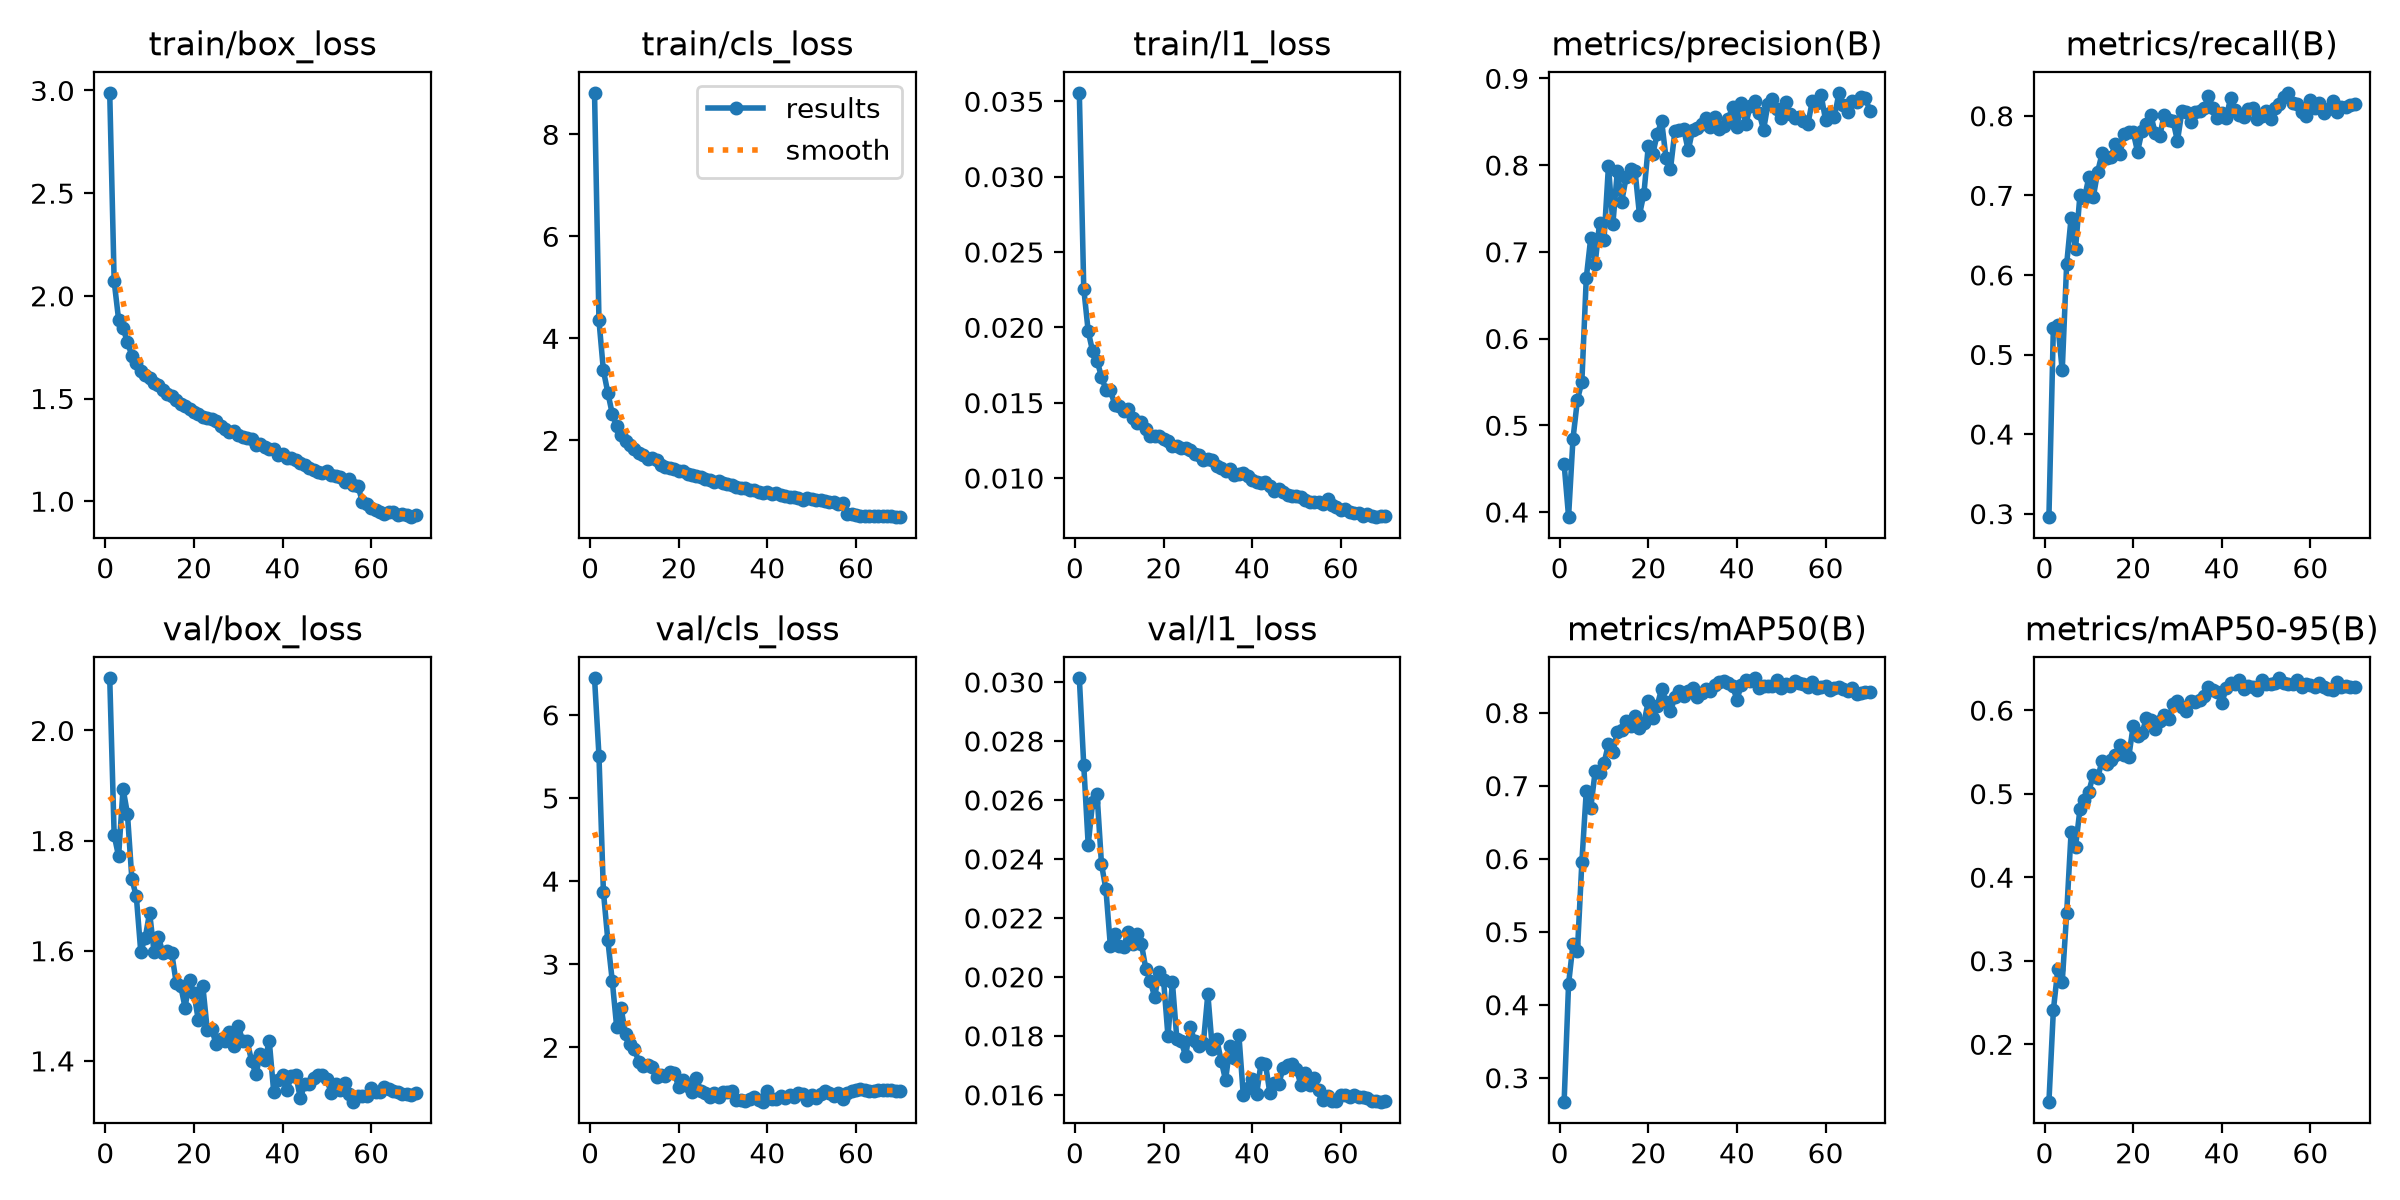
\includegraphics[width=\columnwidth]{yolo26n_p2_v13_results.png}
\caption{Training metrics of the citrus pest and disease detector.}
\end{figure}

Fig. 2 shows the per-class prediction distribution and confusions. At a confidence threshold of 0.25, the test set yields 675 TP, 118 FP, and 135 FN, with a Detection Jaccard of 0.727. Confusions between classes are rare, and misses mostly go to the background, most often for Scale\_Insect (0.37) and Citrus\_Leaf\_Miner (0.36), indicating that small targets and background similarity remain the main limitations. The nine-class test mAP50 of the proposed method is 0.86118, with per-class results in Section 4.5. The valid/test gap of Scale\_Insect is 0.1738, but three training runs on the same data give gaps of 0.040 to 0.174, reflecting its small evaluation sets (35 images each). The TFLite model in the app, whose input is fixed at 640×640, reaches a test mAP50 of 0.857.

\begin{figure}[t]
\centering
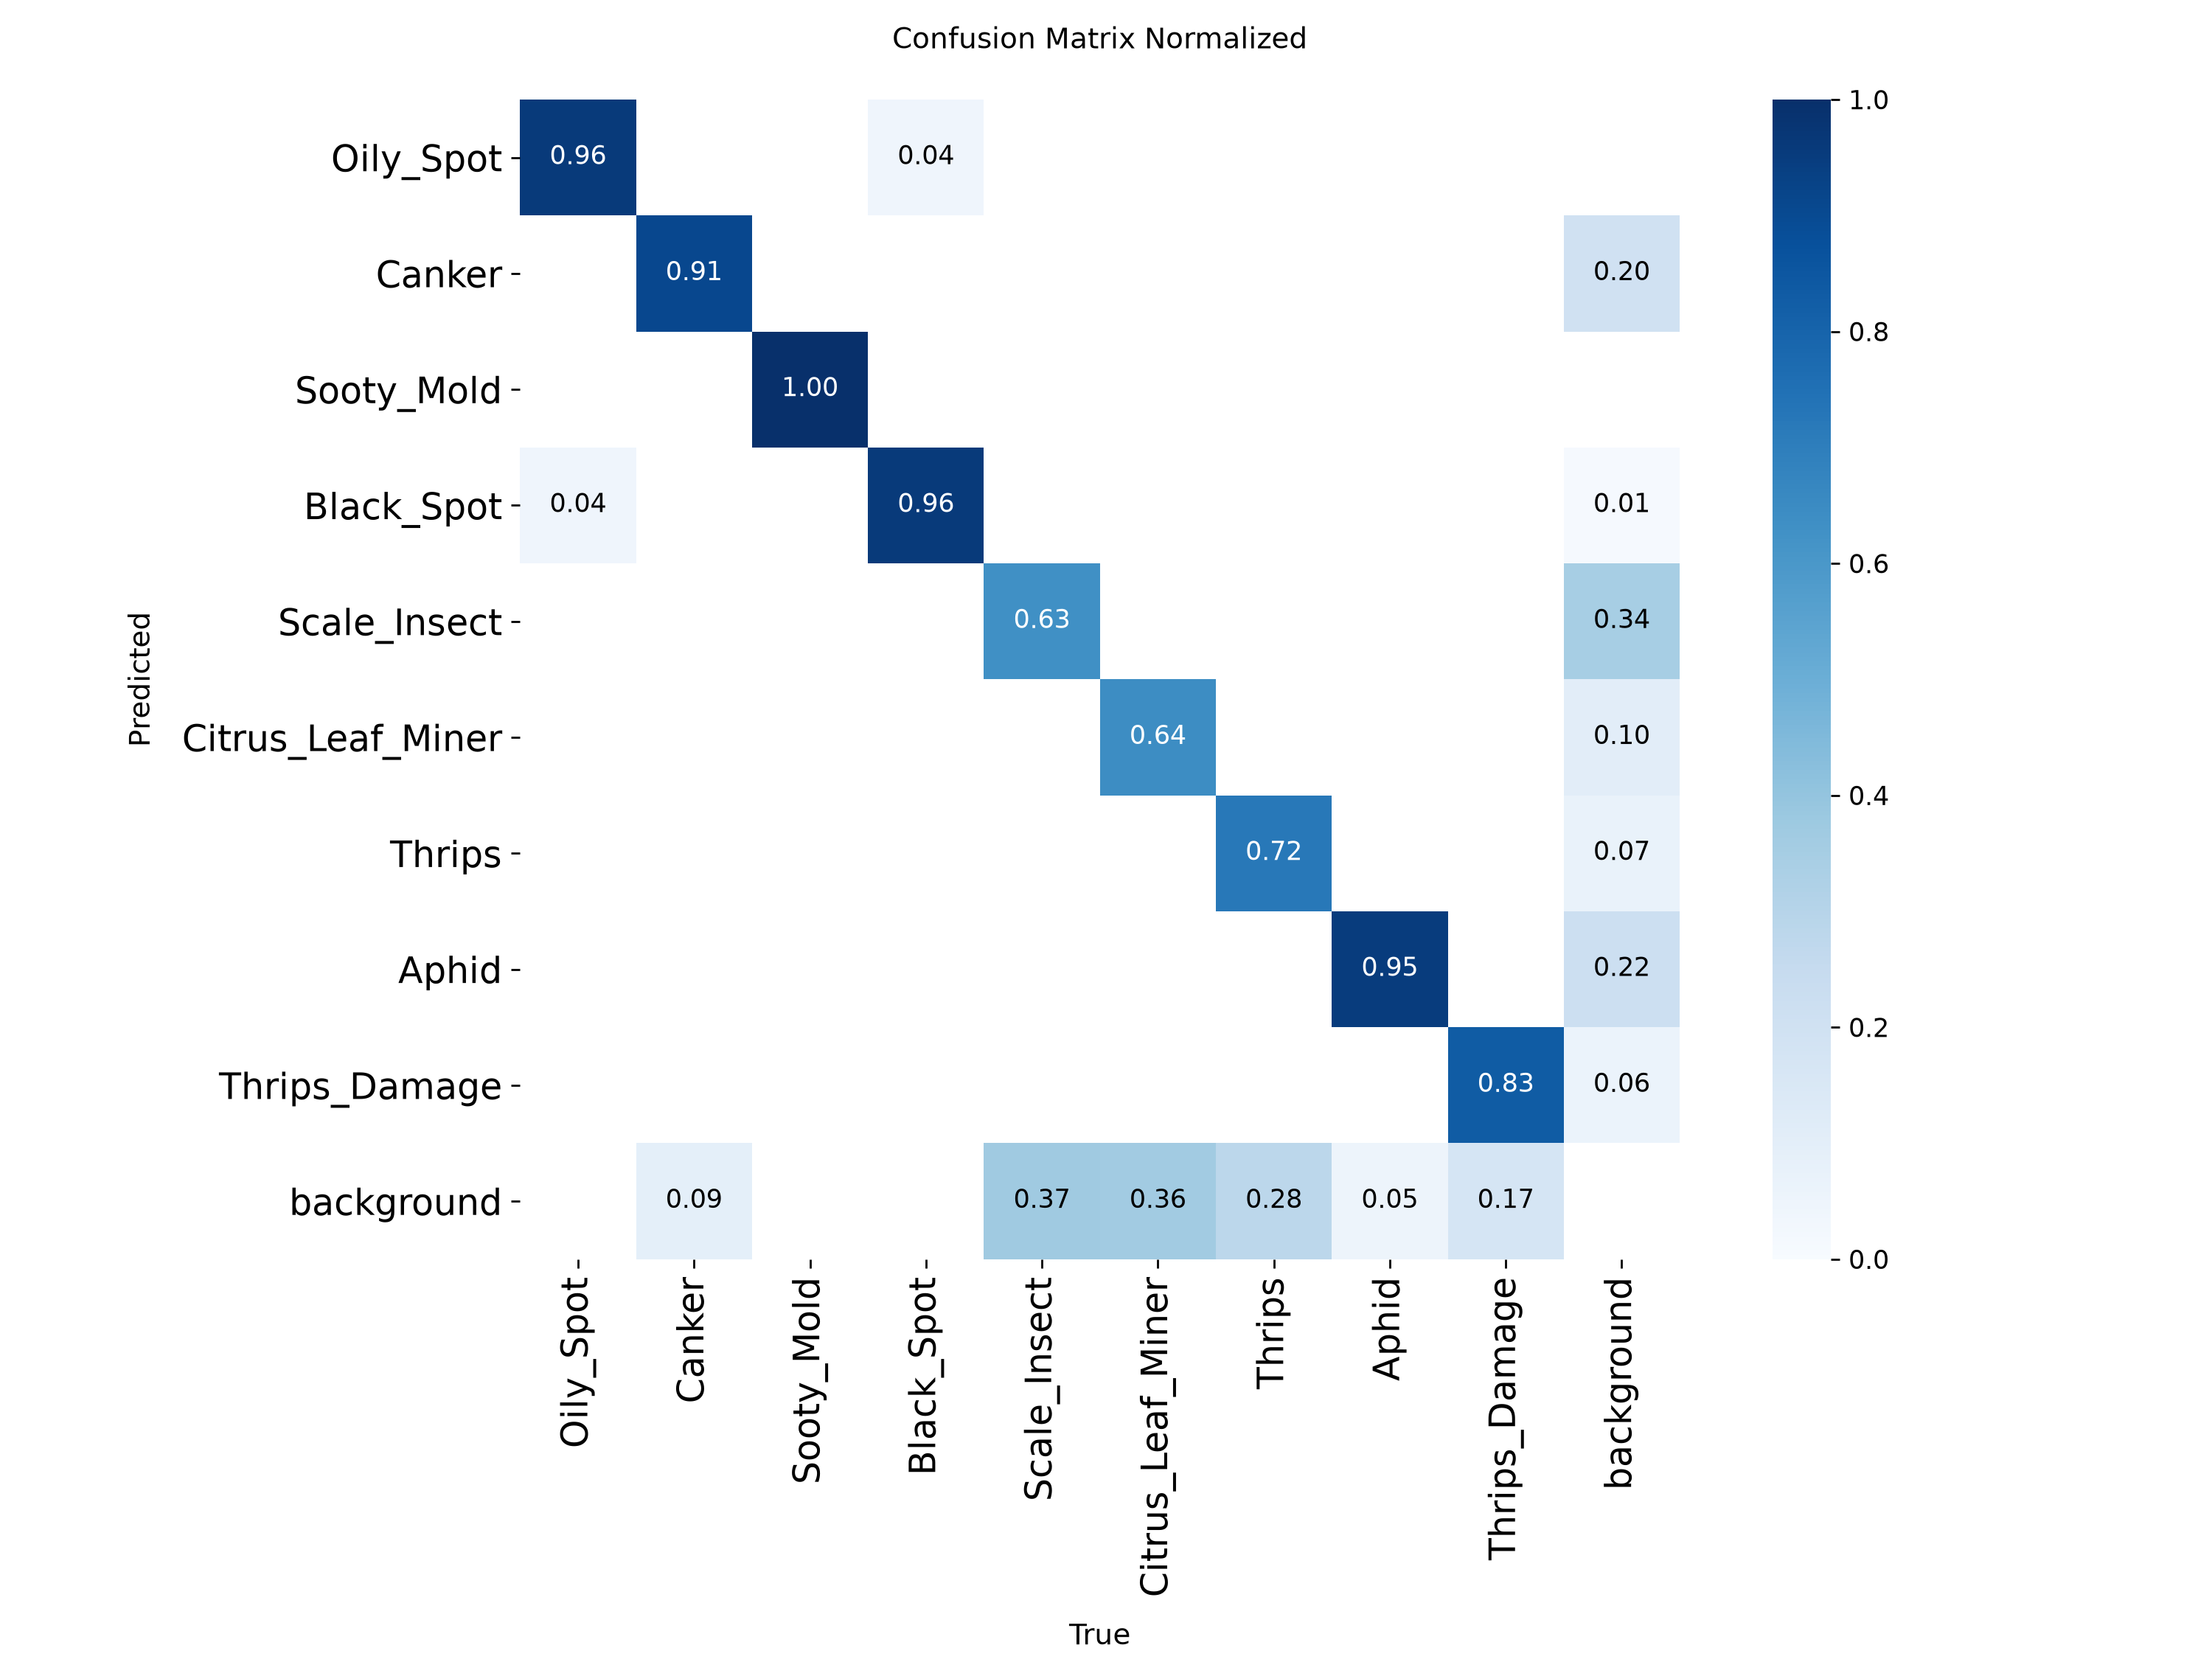
\includegraphics[width=\columnwidth]{yolo26n_p2_v13_confusion_matrix_norm.png}
\caption{Normalized confusion matrix on the test set (confidence threshold 0.25).}
\end{figure}

External detached-leaf images raise the AP50 of Citrus\_Leaf\_Miner by only 0.0209, below the preset gain threshold of 0.04 and comparable to Oily\_Spot (+0.0211), to which no data were added; when the data domain does not match, adding images does not necessarily improve field recognition. The nine-class mAP50 is 0.0516 higher than the 0.8096 obtained under the previous annotation convention, of which 0.0438 comes from the larger Thrips\_Damage boxes (median area from 11.30\% to 15.40\%). The eight unchanged classes average 0.8508 AP50, close to 0.8527 under the previous convention, so the change in the nine-class score cannot be read as an across-the-board gain in model capability.

\subsection{Grounded Diagnosis Results}
% 來源：20260924_citrus_rag_ablation_study.md 表 3-1 階段 5
With all components enabled (atomic chunks, adaptive retrieval, fine-tuning, and guardrail), the full system reaches 85.05\% Faithfulness, 100.0\% Context Precision, and 93.06\% Context Recall on the 40-question benchmark and defends all four boundary questions. Since Context Recall is below 100\%, retrieval can still miss some conditions that an answer requires.

Typical errors include fabricated pathogen names, contraindications mixed up between different pests and diseases, and citrus advice applied to non-citrus crops. Atomic chunks and the answer format reduce the first two, and the safety guardrail refuses cross-crop and non-agricultural questions as well as empty retrievals. With the guardrail disabled, the fine-tuned model fails all four boundary questions and the base model defends only two, showing that safety is a system property formed jointly by the model, retrieval, and application.

\subsection{LLM+RAG Ablation}
% 來源：20260924_citrus_rag_ablation_study.md 表 3-1、§4.1–4.4（Galaxy A33、4 執行緒、Qwen2.5-7B 裁判 T=0.0）
Table 1 lists the five-stage cumulative ablation. Knowledge decoupling contributes the most: the 10 coarse chunks in stage 1 drive the 0.5B model into repetitive output averaging 419.7 tokens, whereas the 33 atomic chunks raise Faithfulness from 22.92\% to 83.86\% and cut the output to 73.6 tokens. Adaptive retrieval, following Pocket RAG~\cite{kang2026}, raises Context Precision from 98.61\% to 100.0\% and Context Recall from 89.58\% to 93.06\%.

\begin{table}[t]
\centering
\caption{Five-stage cumulative ablation of on-device RAG (Galaxy A33, 40 questions; Faith. = Faithfulness, CP = Context Precision, CR = Context Recall, Def. = boundary defense rate; total latency in seconds, others in \%).}
\small
\begin{tabular}{@{}lccccc@{}}
\toprule
\textbf{Stage} & \textbf{Faith.} & \textbf{CP} & \textbf{CR} & \textbf{Def.} & \textbf{Total} \\
\midrule
1 Baseline & 22.92 & 75.00 & 44.91 & 0 & 37.08 \\
2 +Atomic chunks & 83.86 & 98.61 & 89.58 & 0 & 21.55 \\
3 +Adaptive retrieval & 82.64 & 100.0 & 93.06 & 50 & 22.61 \\
4 +SFT & 87.04 & 100.0 & 93.06 & 0 & 30.85 \\
5 +Guardrail & 85.05 & 100.0 & 93.06 & 100 & 29.98 \\
\bottomrule
\end{tabular}
\end{table}

Supervised fine-tuning raises Faithfulness from 82.64\% to 87.04\%, a net gain of 4.40 percentage points, and the PREP compliance rate from 15.00\% to 22.50\%. The output grows from 90.0 to 163.2 tokens, increasing the total latency, while decoding speed drops from 9.66 to 9.40 tok/s, indicating that fine-tuning mainly improves evidence following and prescription completeness rather than native decoding capability. However, fine-tuning also makes the model answer cross-crop and non-agricultural questions with citrus knowledge: without the guardrail, the defense rate falls from 50\% to 0\%, and with the guardrail it reaches 100\%. Faithfulness in stage 5 is 1.99 percentage points lower than in stage 4; because each stage was measured only once, this is insufficient to conclude that the guardrail reduces faithfulness.

\subsection{Mobile Performance and Limitations}
% 來源：ablation study 表 3-1；20260729_mobile_rag_benchmark.md §2；detection docs/v13_報告 §4、v5.7_報告 §3.4
On the Galaxy A33 with 4 threads, the 40-question evaluation has a mean TTFT of 13.75 s, a decoding speed of 9.56 tok/s, and a total latency of 29.98 s per question. In a pure-SLM test of an early prototype, 6 threads reduced TTFT from 2,613.1 ms to 2,110.3 ms and raised decoding speed from 10.40 to 13.70 tok/s, but the delivered version keeps 4 threads to balance power consumption and heat. Sustained vision inference reaches 38.4 FPS at 320 pixels on a Dimensity 8300 and 29.8 FPS on a Snapdragon 8 Gen 2, whereas the Snapdragon 662 fails the combined accuracy and latency gate. These measurements used earlier weights of the same architecture, so the latency carries over, but the accuracy must be re-evaluated with the delivered weights. The app therefore adopts photo-based recognition, and real-time streaming is left as a future feature.

Limitations include a single random seed per detection experiment, an annotation-consistency study of only 20 images, a single run per RAG ablation stage on one phone, no joint evaluation of the detection and question-answering modules yet, and chemical-treatment text that still needs review by experts and against official pesticide labels.

\subsection{Class-Level Results and Data Quality}
% 來源：detection docs/v5.7_報告 §3.1 第 1 點
To keep the overall mAP from masking class differences, this study reports the pooled AP50 of all nine classes. Sooty\_Mold, Black\_Spot, and Oily\_Spot, whose visual features are more distinctive, reach 0.9950, 0.9528, and 0.9482, and Aphid and Canker reach 0.9297 and 0.9045; Thrips\_Damage, Citrus\_Leaf\_Miner, Thrips, and Scale\_Insect reach 0.7848, 0.7403, 0.7040, and 0.6321. The latter four involve small targets, occlusion, shape variation, or background similarity, and future data collection should first add samples from different growth stages and camera distances.

Data acceptance covers image–label pairing, class IDs, coordinate bounds, data leakage, near-duplicates across subsets, box-area ratios after augmentation, and absolute evaluation-set counts. All nine pooled two-standard-error upper bounds are at most 0.10, the largest being 0.099 for Citrus\_Leaf\_Miner. Although these checks cannot replace repeated training, they help distinguish data-quality problems from random model variation. The rise in annotation consistency from 0.746 to 0.899 also shows that the evaluation unit of an image task must first be defined by domain knowledge; the measured consistency after relabeling the whole class is 0.80 to 0.83.

\subsection{Question-Answering Evaluation and Error Analysis}
% 來源：ablation study §2.5–2.6；citrus-ragas-eval docs/academic_ragas_evaluation_methodology.md
The Pilot evaluation is used to find prompt echoing, fabricated scientific names, cross-crop hallucination, and answer-format problems, and the Full Benchmark tests the formal system with 36 citrus-domain questions and 4 boundary questions. Scoring uses Qwen2.5-7B-Instruct outside the phone as the judge (temperature 0): each answer is split into atomic statements, which are judged as supported or unsupported by the retrieved content, and pesticides, dilution ratios, or symptoms not recorded in the chunks are treated as unsupported~\cite{es2023}. Faithfulness is the proportion of supported statements, Context Precision measures whether the top-ranked chunk is relevant, and Context Recall measures whether the information needed by the reference answer is covered; this design suits structured agricultural answers better than exact string matching.

Error analysis shows that a correct detection does not guarantee a safe diagnostic text. When pathogen, pesticide, and crop names are similar, a short context may lead the model to merge two entities, and for low-information questions such as “the leaves are turning yellow,” the model may give treatment advice beyond the evidence. Answers must therefore present the recognition result, retrieved evidence, and unverified status together while retaining human review; chemical treatments should not be inferred by the model but referred to official labels or agricultural experts.

\subsection{On-Device Workflow and Engineering Trade-offs}
% 來源：citrus-rag-mobile rag_orchestrator_service.dart；report RAG向量資料庫/架構設計.md §1、§6.3；ablation study §3.2
The workflow has six steps—image input, candidate detection, user follow-up questions, safety checking, knowledge retrieval, and answer generation—and images and conversations are processed entirely on the phone. The knowledge base (about 30 KB) is loaded as a built-in app asset, whereas the 379 MB model weights are stored in the app sandbox and loaded with mmap to reduce memory pressure. Retrieval takes about 10.18 ms on average, only 0.03\% of the total latency per question, so optimization should focus on model loading, prompt prefill, context length, and answer caching.

On the Galaxy A33, TTFT accounts for about 46\% of the total latency per question, and prompt prefill is the main bottleneck. The 2,110.3 ms measured on the early prototype with short prompts of 30 to 250 characters follows a different protocol, and the two should not be merged into a single product latency. Low-end devices are better suited to photo-based recognition than to continuous streaming, and high-end devices should also be judged by sustained load rather than a single peak FPS.

\subsection{Experimental Control and Interpretation}
This study controls data quality, model capability, and application performance separately. Detection experiments fix the data split and input size and report both the nine-class and the unchanged eight-class results, so that a change in the boxing rule of one class is not mistaken for an overall model improvement. The external-image experiment fixes the total number of training images and changes only the source and background of some images to determine whether a gain comes from sample count or domain similarity; the results show that detached-leaf images on white paper cannot directly replace orchard images.

The detection metrics must also be distinguished: mAP50 is the mean average precision at IoU=0.5, and mAP50–95 is stricter on localization; Precision reflects false alarms and Recall reflects misses, while the Jaccard from the confusion matrix is computed at a fixed confidence threshold, so they should not be treated as equivalent in the same table. For agricultural users, low Recall may miss small pests and low Precision may cause unnecessary manual inspection; the deployment threshold should therefore be adjusted to the use case rather than tuned for a single highest score.

Question-answering evaluation is likewise interpreted in layers. Reporting Faithfulness, Context Precision, and Context Recall together separates three failure types: correct retrieval with an out-of-bounds answer, missed retrieval, and a model that does not follow the evidence. The boundary questions test whether the system stops generating when evidence is insufficient, a safety metric that cannot be omitted in agricultural treatment scenarios.

\subsection{Use Scenario and Risk Management}
% 來源：OneLeaf-dx/APP README.md（功能與架構）；citrus-rag-mobile rag_orchestrator_service.dart（0-Hit 回覆）
After the user photographs a leaf or selects an image from the album, the system returns candidate pests and diseases, confidence scores, and bounding boxes and opens a conversation with the highest-confidence candidate, after which the user can ask about symptoms or management. On-device retrieval selects chunks by crop, pest or disease, symptom, and question terms; if no chunk passes the thresholds, the system reports that no high-confidence knowledge was found and suggests consulting local experts instead of offering general language-model knowledge as formal control advice. Answers should retain an evidence summary so that users can trace the source of a recommendation.

Risk management has three layers. The data layer documents different crops, pests and diseases, and application conditions separately to prevent cross-contamination of chunks; the model layer uses fine-tuning and structured output to reduce fabricated names, repetitive sentences, and cross-entity confusion; and the application layer stops when retrieval is empty or a question is cross-crop or non-agricultural, while labeling chemical names and unverified treatments is left for future work. All three layers are necessary, because even a well-trained model may meet situations that the database does not cover.

The system is positioned as an offline tool for preliminary screening and evidence navigation, not for automatic prescription. Farmers can decide from the recognition result whether to capture additional views or seek professional help, and agricultural staff can use bounding boxes, candidate classes, and source chunks to speed up initial assessment. Formal pesticide use must still be checked against announcements of the Ministry of Agriculture~\cite{moa2026}, product labels, the registered crop and pest scope, the application concentration, and the pre-harvest interval.

\subsection{Reproducibility and Future Work}
For reproducibility, this study records the dataset split, image and box counts, annotation rules, near-duplicate checking method, training settings, confidence threshold, knowledge-chunk version, question set, judging rules, device model, and thread count. After every update of the data or knowledge base, leakage checks, class-level evaluation, boundary questions, and long-duration load tests should be rerun; updating only the model weights without revalidating the knowledge base cannot guarantee safe answers, and updating only the knowledge base may also change the answer distribution and latency.

Future work has four directions: (1) repeating the detection and RAG experiments at least three times across more phones and crops and reporting means with bootstrap confidence intervals; (2) extending the annotation-consistency study to all nine classes, different imaging conditions, and symptom severities; (3) collecting orchard images from the same domain as the training data and evaluating cross-orchard generalization with a farm-level split; and (4) having two agricultural experts review all chemical-treatment statements and reporting model faithfulness and practical correctness separately. These steps would move the work from engineering verification to field-deployment validation.

\section{Conclusion}
This study presented a fully on-device method for citrus pest and disease recognition and grounded diagnosis. The detector achieves an mAP50 of 0.861 and an mAP50–95 of 0.641 on the nine-class test set, and the on-device RAG reaches 85.05\% Faithfulness, 100.0\% Context Precision, and 93.06\% Context Recall on the 40-question benchmark while defending cross-crop and out-of-domain boundary questions. The ablation shows that knowledge-chunk granularity has the largest effect and that the fine-tuned model must be paired with a guardrail. Overall, annotation consistency, domain similarity, retrieval evidence, and safety guardrails affect system reliability no less than the model architecture. The method can serve as a foundation for offline agricultural assistance tools, but control advice should still follow official labels and the judgment of agricultural professionals.

\section*{Acknowledgement}
This work was partially supported by the National Science and Technology Council, Taiwan, under grant NSTC 115-2221-E-025-006.

% references follow the Chinese version: original citation order, IEEE style, verified entry by entry
{\small
\begin{thebibliography}{23}
\bibitem{mohanty2016} S. P. Mohanty, D. P. Hughes, and M. Salathé, “Using deep learning for image-based plant disease detection,” \textit{Frontiers in Plant Science}, vol. 7, p. 1419, 2016.
\bibitem{ferentinos2018} K. P. Ferentinos, “Deep learning models for plant disease detection and diagnosis,” \textit{Computers and Electronics in Agriculture}, vol. 145, pp. 311–318, 2018.
\bibitem{kamilaris2018} A. Kamilaris and F. X. Prenafeta-Boldú, “Deep learning in agriculture: A survey,” \textit{Computers and Electronics in Agriculture}, vol. 147, pp. 70–90, 2018.
\bibitem{pacal2024} I. Pacal, I. Kunduracioglu, M. H. Alma, M. Deveci, S. Kadry, J. Nedoma, V. Slany, and R. Martinek, “A systematic review of deep learning techniques for plant diseases,” \textit{Artificial Intelligence Review}, vol. 57, no. 11, p. 304, 2024.
\bibitem{moa2026} Ministry of Agriculture, Taiwan, “Ministry of agriculture official website,” [Online]. Available: \url{https://www.moa.gov.tw/}, 2026. Accessed: 2026-07-02.
\bibitem{hughes2015} D. P. Hughes and M. Salathé, “An open access repository of images on plant health to enable the development of mobile disease diagnostics,” arXiv preprint arXiv:1511.08060, 2015.
\bibitem{guan2023} H. Guan, C. Fu, G. Zhang, K. Li, P. Wang, and Z. Zhu, “A lightweight model for efficient identification of plant diseases and pests based on deep learning,” \textit{Frontiers in Plant Science}, vol. 14, p. 1227011, 2023.
\bibitem{xiong2024} H. Xiong, J. Li, T. Wang, F. Zhang, and Z. Wang, “EResNet-SVM: An overfitting-relieved deep learning model for recognition of plant diseases and pests,” \textit{Journal of the Science of Food and Agriculture}, vol. 104, no. 10, pp. 6018–6034, 2024.
\bibitem{ashurov2025} A. Y. Ashurov, M. S. A. M. Al-Gaashani, N. A. Samee, R. Alkanhel, G. Atteia, H. A. Abdallah, and M. Saleh Ali Muthanna, “Enhancing plant disease detection through deep learning: A depthwise CNN with squeeze and excitation integration and residual skip connections,” \textit{Frontiers in Plant Science}, vol. 15, p. 1505857, 2025.
\bibitem{xu2023} Y. Xu, Z. Gao, Y. Zhai, Q. Wang, Z. Gao, Z. Xu, and Y. Zhou, “A CNNA-based lightweight multi-scale tomato pest and disease classification method,” \textit{Sustainability}, vol. 15, no. 11, p. 8813, 2023.
\bibitem{goyal2025} A. Goyal and K. Lakhwani, “Integrating advanced deep learning techniques for enhanced detection and classification of citrus leaf and fruit diseases,” \textit{Scientific Reports}, vol. 15, p. 12659, 2025.
\bibitem{he2016} K. He, X. Zhang, S. Ren, and J. Sun, “Deep residual learning for image recognition,” in \textit{Proc. CVPR}, pp. 770–778, 2016.
\bibitem{deng2009} J. Deng, W. Dong, R. Socher, L.-J. Li, K. Li, and L. Fei-Fei, “ImageNet: A large-scale hierarchical image database,” in \textit{Proc. CVPR}, pp. 248–255, 2009.
\bibitem{lin2017} T.-Y. Lin, P. Goyal, R. Girshick, K. He, and P. Dollár, “Focal loss for dense object detection,” in \textit{Proc. ICCV}, pp. 2980–2988, 2017.
\bibitem{selvaraju2017} R. R. Selvaraju, M. Cogswell, A. Das, R. Vedantam, D. Parikh, and D. Batra, “Grad-CAM: Visual explanations from deep networks via gradient-based localization,” in \textit{Proc. ICCV}, pp. 618–626, 2017.
\bibitem{shorten2019} C. Shorten and T. M. Khoshgoftaar, “A survey on image data augmentation for deep learning,” \textit{Journal of Big Data}, vol. 6, no. 1, p. 60, 2019.
\bibitem{feng2025} W. Feng, J. Liu, Z. Li, and S. Lyu, “YOLO-Citrus: A lightweight and efficient model for citrus leaf disease detection in complex agricultural environments,” \textit{Frontiers in Plant Science}, vol. 16, p. 1668036, 2025, doi: 10.3389/fpls.2025.1668036.
\bibitem{hu2021} E. J. Hu, Y. Shen, P. Wallis, Z. Allen-Zhu, Y. Li, S. Wang, L. Wang, and W. Chen, “LoRA: Low-rank adaptation of large language models,” arXiv preprint arXiv:2106.09685, 2021.
\bibitem{qwen2025} Qwen Team, “Qwen2.5 technical report,” arXiv preprint arXiv:2412.15115, 2025.
\bibitem{kang2026} D. H. Kang, H. Lee, H. Cha, M. Choi, and S. Lim, “Pocket RAG: On-device RAG for first aid guidance in offline mobile environment,” arXiv preprint arXiv:2602.13229, 2026.
\bibitem{guainazzo2026} N. Guainazzo, G. Delzanno, D. Ancona, and D. D’Agostino, “Navigating the Seas of AI: Effectiveness of small language models on edge devices for maritime applications,” \textit{Sensors}, vol. 26, no. 5, p. 1590, 2026, doi: 10.3390/s26051590.
\bibitem{rafailov2023} R. Rafailov, A. Sharma, E. Mitchell, C. D. Manning, S. Ermon, and C. Finn, “Direct preference optimization: Your language model is secretly a reward model,” in \textit{Advances in Neural Information Processing Systems}, vol. 36, pp. 53728–53741, 2023.
\bibitem{es2023} S. Es, J. James, L. Espinosa-Anke, and S. Schockaert, “RAGAS: Automated evaluation of retrieval augmented generation,” arXiv preprint arXiv:2309.15217, 2023.
\end{thebibliography}
}

\end{document}
